\graphicspath{
  {./images/bmps/}{./images/vects/}{./images/}
  {./images/presentation/bmps/}{./images/presentation/vects/}{./images/presentation/}
  {./images/chapter00/bmps/}{./images/chapter00/vects/}{./images/chapter00/}
  {./images/chapter02/bmps/}{./images/chapter02/vects/}{./images/chapter02/}
}

\subsection{Non-Rigid Contour Tracking}

\begin{frame}[plain]{Pipeline}
  \begin{columns}[c] % the "c" option specifies center vertical alignment
    \column{.3\textwidth} % column designated by a command
      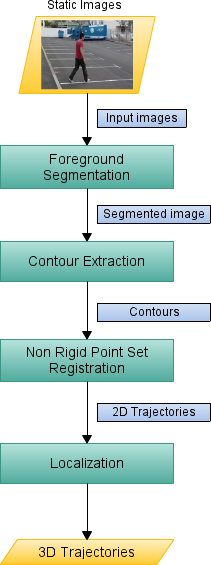
\includegraphics[height=1.1\textheight]{pipeline_cp02}
    \column{.7\textwidth}
      \vspace{-1cm}
      \begin{figure}[t]
	\centering
	\begin{subfigure}[b]{0.3\columnwidth}
	    
\includegraphics[width=\textwidth]{fig17}
	\end{subfigure}% 
	~
	\begin{subfigure}[b]{0.3\columnwidth}
	    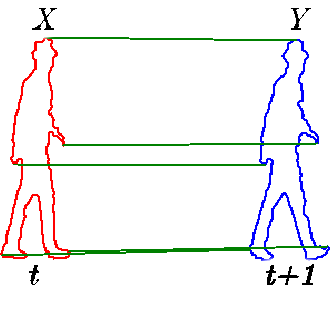
\includegraphics[width=\textwidth]{twoSets2}
	\end{subfigure}%    
	~
	\begin{subfigure}[b]{0.3\columnwidth}
	    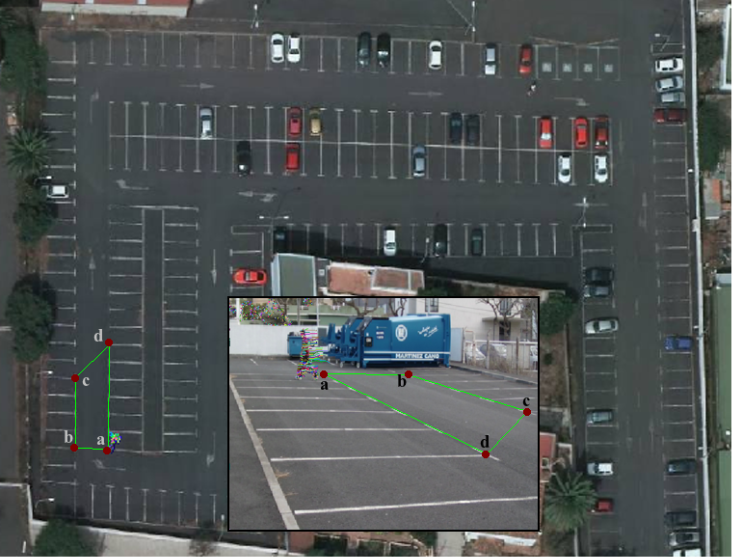
\includegraphics[width=\textwidth]{localization}
	\end{subfigure}%
	\\~\\
	\begin{subfigure}[b]{0.5\columnwidth}
	    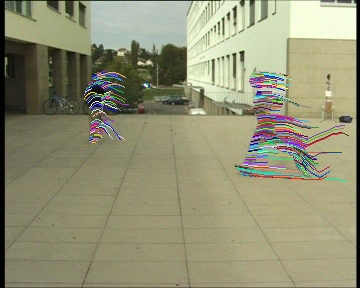
\includegraphics[width=\textwidth]{fig6}
	\end{subfigure}% 
    \end{figure}
  \end{columns}

%   \begin{center}
%     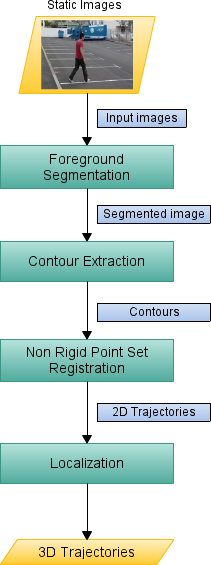
\includegraphics[height=0.7\textheight]{pipeline_cp02}
%   \end{center}
  
  \note {
  \begin{itemize}
    \item First step: Silhouettes of the obstacles are extracted.
    \item Points are extracted from the contours of the masks.
    \item Points are used as input for a Non-Rigid Point Set Registration algorithm.
    \item Matches are used to track the points along the frames.
    \item Paths are projected in the map.
  \end{itemize}
  }
\end{frame}

% \begin{frame}{Foreground extraction}
%   \begin{itemize}
%     \item<1-> BACKground Stochastic Approximation (BACKSA) \citep{lopez2011stochastic}
%     \item<2-> Foreground detection with Self-Organizing Maps (FSOM) \citep{lopez2011foreground}
%     \item<3-> Hierarchical Foreground Detector \citep{guo2011hierarchical}
%     \item<4-> Block-based Classifier Cascade with Probabilistic Decision Integration (BCCPDI) \cite{reddy2012improved}
%   \end{itemize}
% %   \begin{overlayarea}{\textwidth}{\textheight}
% %       \only<1>{
% %       \begin{block}{BACKground Stochastic Approximation (BACKSA)}
% % 	\begin{itemize}
% % 	  \item Statistical approach for background modeling and foreground segmentation.
% % 	  \item Dual mixture model at each pixel location models the foreground and background distributions
% %  	  \item A learning algorithm with a low complexity is used
% % 	\end{itemize}
% % 	\note{
% % 	  \begin{itemize}
% % 	    \item Statistical approach for bg modeling and fg segmentation
% % 	    \item Dual mixture model at each px location models the fg and bg distributions
% % 	    \begin{itemize}
% % 	      \item bg, a Gaussian distribution is used
% % 	      \item fg, modeled by a uniform distribution
% % 	    \end{itemize}
% % 	    \item Learning model is used
% % 	  \end{itemize}	
% % 	}
% %       \end{block}
% %       }
% %       \only<2>{
% %       \begin{block}{Foreground detection with Self-Organizing Maps (FSOM)}
% % 	\begin{itemize}
% % 	  \item Neural network based alternative
% % 	  \item Background is modeled using probabilistic self-organizing maps
% % 	  \item A statistic correlation measure is also used
% % 	\end{itemize}
% % 	\note{
% % 	  \begin{itemize}
% % 	    \item Neural network based alternative
% % 	    \item Background is modeled using probabilistic self-organizing maps
% % 	    \item A statistic correlation measure is also used (to test the similarity among nearby pixels)
% % 	    \item This measure provides feedback to the process
% % 	  \end{itemize}	
% % 	}
% %       \end{block}
% %       }
% %       \only<3>{
% %       \begin{block}{Hierarchical Foreground Detector (hierFG)}
% % 	\begin{itemize}
% % 	  \item Hierarchical scheme supported by block-based and pixel-based codebooks
% % 	  \begin{itemize}
% % 	    \item Block Truncation Coding is extended
% % 	  \end{itemize}
% % 	  \item Block-based background modeling
% % 	  \item Pixel-based codebook
% % 	  \item Good performance even when background is not completely still
% % 	\end{itemize}
% % 	\note{
% % 	  \begin{itemize}
% % 	    \item Uses a hierarchical scheme supported by block-based and pixel-based codebooks
% % 	    \item Block Truncation Coding (a traditional compression scheme) is extended (dividing the image in multiple non-overlapped blocks, representing them w/ a set of 12 intensity values)
% % 	    \item Block-based background modeling: foreground is efficiently detected, but with low precision.
% % 	    \item Pixel-based codebook: enhances accuracy (w/o decressing processing speed)
% % 	    \item Good performance even when background is not completely still
% % 	  \end{itemize}	
% % 	}
% %       \end{block}
% %       }
% %       \only<4>{
% %       \begin{block}{Block-based Classifier Cascade with Probabilistic Decision Integration (BCCPDI)}
% % 	\begin{itemize}
% % 	  \item An image is divided into overlapping blocks
% % 	  \item Cascade Classifier
% % 	  \item Generation of a foreground mask
% % 	\end{itemize}
% % 	\note{
% % 	  Sequences are analyzed as overlapped blocks
% % 	  \begin{enumerate}
% % 	    \item An image is divided into overlapping blocks ( for each block, a low-dimensional texture descriptor is generated and passed to a cascade classifier)
% % 	    \item (Each block is classified as bg or fg using the) Cascade Classifier (three classifiers:
% % 	    \begin{enumerate}
% % 	      \item Able to handle dynamic bg
% % 	      \item Detects if anomalies found are generated by illumination changes
% % 	      \item Able to exploit temporal correlations
% % 	    \end{enumerate}
% % 	    \item  ( A probabilistic approach for the) Generation of a foreground mask (which exploits the block overlaps)
% % 	  \end{enumerate}	
% % 	}
% %       \end{block}
% %       }
% %   \end{overlayarea}
% \end{frame}
% 
% \begin{frame}{Contour flow detection}
%   \begin{center}
%     \includegraphics[height=0.7\textheight]<1>{twoSets1}
%     \includegraphics[height=0.7\textheight]<2>{twoSets2}
%   \end{center}
% \end{frame}
% 
% \begin{frame}{Contour flow detection}
%   \begin{itemize}
%     \item<1-> Iterated Closest Point (ICP) \citep{besl1992method, feldmar1996rigid}
%     \item<2-> Thin-Plate Splines Robust Point Matching (TPS-RPM) \citep{chui2000new}
%     \item<3-> Coherent Point Drift (CPD) \citep{myronenko2010point}
%     \item<4-> Robust Point Matching for Non-Rigid Shapes (RPM-NRS) \citep{zheng2006robust}
%     \item<5-> Dynamic Programming based Point Set Matching (DPPSM-MST, DPPSM-STAR) \cite{lian2012rotation}
%   \end{itemize}
% %   \begin{overlayarea}{\textwidth}{\textheight}
% %       \only<1>{
% %       \begin{block}{Iterated Closest Point (ICP)}
% % 	\begin{itemize}
% % 	  \item Improved version which allows non-rigid surface registration
% % 	\end{itemize}
% % 	\note{
% % 	  
% % 	}
% %       \end{block}
% %       }
% %       \only<2>{
% %       \begin{block}{Thin-Plate Splines Robust Point Matching (TPS-RPM)}
% % 	\begin{itemize}
% % 	  \item Uses a Thin-Plate Spline (TPS) kernel
% % 	  \item Alternates the update and correspondence parameters
% % 	\end{itemize}
% % 	\note{
% % 	  \begin{itemize}
% % 	    \item (Uses a TPS Kernel that contains info about the point sets internal structural relationships) and generates a non-rigid warp
% % 	    \item Alternates the update (of the mapping) and correspondence parameters (in the way that both solutions mutually improve one another during the process until convergence is reached)
% % 	  \end{itemize}	
% % 	}
% %       \end{block}
% %       }
% %       \only<3>{
% %       \begin{block}{Coherent Point Drift (CPD)}
% % 	\begin{itemize}
% % 	  \item Multidimensional probabilistic robust registration method
% % 	  \item Able to deal with rigid and non-rigid point sets
% % 	  \item Defines the alignment of two point sets as a PDE problem
% % 	  \item Advantages:
% % 	  \begin{itemize}
% % 	    \item Able to register non-rigid large data sets
% % 	    \item Reduced number of free parameters and iterations
% % 	    \item Robust and accurate performance with respect to noise, outliers and missing points.
% % 	  \end{itemize}
% % 	\end{itemize}
% % 	\note{
% % 	  \begin{itemize}
% % 	    \item Multidimensional probabilistic robust registration method
% % 	    \item Able to deal with rigid and non-rigid point sets
% % 	    \item Defines the alignment of two point sets as a probability density estimation problem
% % 	    \item Advantages:
% % 	    \begin{itemize}
% % 	      \item Able to register non-rigid large data sets
% % 	      \item Reduced number of free parameters and iterations (and processing time --> The estimation of the GMM width reduces the number of iterations and the processing time)
% % 	      \item (Compared to other methods) Robust and accurate performance with respect to noise, outliers and missing points.
% % 	    \end{itemize}
% % 	  \end{itemize}	
% % 	}
% %       \end{block}
% %       }
% %       \only<4>{
% %       \begin{block}{Robust Point Matching for Non-Rigid Shapes (RPM-NRS)}
% % 	\begin{itemize}
% % 	  \item Each point is considered a node in the graph
% % 	  \item Two nodes are connected by an edge only if they are neighbors
% % 	  \item Problem becomes a maximization problem
% % 	\end{itemize}
% % 	\note{
% % 	  \begin{itemize}
% % 	    \item Each point is considered a node in the graph
% % 	    \item Two nodes are connected by an edge only if they are neighbors
% % 	    \item Problem becomes a maximization problem
% % 	  \end{itemize}		
% % 	}
% %       \end{block}
% %       }
% %       \only<5>{
% %       \begin{block}{Dynamic Programming based Point Set Matching (DPPSM)}
% % 	\begin{itemize}
% % 	  \item Also a graph is constructed from the point set
% % 	  \item Edges are used to determine the orientations of Shape Context (SC) descriptors
% % 	  \item \emph{Data point set} $\rightarrow$ a complete graph is used
% % 	  \item \emph{Model point set} $\rightarrow$ two different approaches:
% % 	  \begin{itemize}
% % 	    \item Minimum Spanning Tree (DPPSM-MST)
% % 	    \item Star Graph (DPPSM-STAR)
% % 	  \end{itemize}
% % 	\end{itemize}
% % 	\note{
% % 	  \begin{itemize}
% % 	    \item Also a graph is constructed from the point set
% % 	    \item Edges are used to determine the orientations of Shape Context (SC) descriptors
% % 	    \begin{itemize}
% % 	      \item SCs can be regarded as the atributes of the edges
% % 	    \end{itemize}
% % 	    \item Data point set: a complete graph is used
% % 	    \item Model point set: two different approaches:
% % 	    \begin{itemize}
% % 	      \item Minimum Spanning Tree (DPPSM-MST)
% % 	      \item Star Graph (DPPSM-STAR)
% % 	    \end{itemize}
% % 	  \end{itemize}
% % 	}
% %       \end{block}
% %       }
% %   \end{overlayarea}
% \end{frame}
% 
% \begin{frame}{Points matching}
%   \begin{itemize}
%    \item Matches are filtered in order to avoid that a point belonging to an object is matched with a point from other.
%    \begin{enumerate}
%     \item $X$ and $Y$ are clustered into different objects using the method in chapter 6.2 of \cite{rusu2009semantic}\\ \begin{center}
%       $\mathcal{C_X} = \{ X_i ~|~ i=1 \dots M \}$, $\mathcal{C_Y} = \{ Y_j ~|~ i=j \dots N \}$.
%     \end{center}
%     \item For each cluster $X_i$ we define a squared region $Rx_i$.
%     \item Each region $Rx_i$ is compared with each region $Ry_j$ \citep{siebel2003design} $\rightarrow$ $\varDelta x$, $\varDelta y$, $\varDelta w$, $\varDelta h$. Then,\\
%     \begin{center}
%      $\delta (Rx_i, Ry_j) = \alpha_1 \varDelta x + \alpha_2 \varDelta y + \alpha_3 \varDelta w + \alpha_4 \varDelta h$
%     \end{center}
%     \item Based on the score, we label the points and reject invalid matches.
%    \end{enumerate}
%   \end{itemize}
% \end{frame}
% 
% \begin{frame}{Points matching}
%   \begin{center}
%    \begin{figure}[t]
%       \begin{subfigure}[b]{0.32\textwidth}
% 	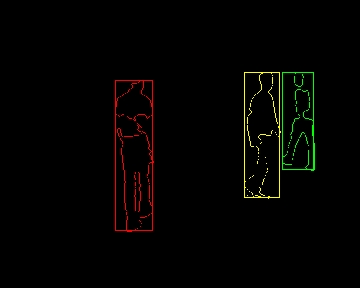
\includegraphics[width=\textwidth]{fig1.jpg}
%       \end{subfigure}%        
%       ~
%       \begin{subfigure}[b]{0.32\textwidth}
% 	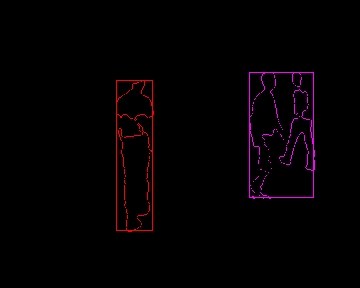
\includegraphics[width=\textwidth]{fig2.jpg}
%       \end{subfigure}%
%       ~
%       \begin{subfigure}[b]{0.32\textwidth}
% 	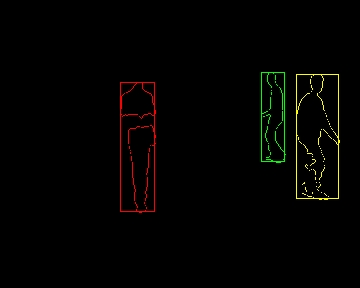
\includegraphics[width=\textwidth]{fig3.jpg}
%       \end{subfigure}%
%     \end{figure}
%   \end{center}
% \end{frame}
% 
% \begin{frame}{Points matching}
%   \begin{center}
%     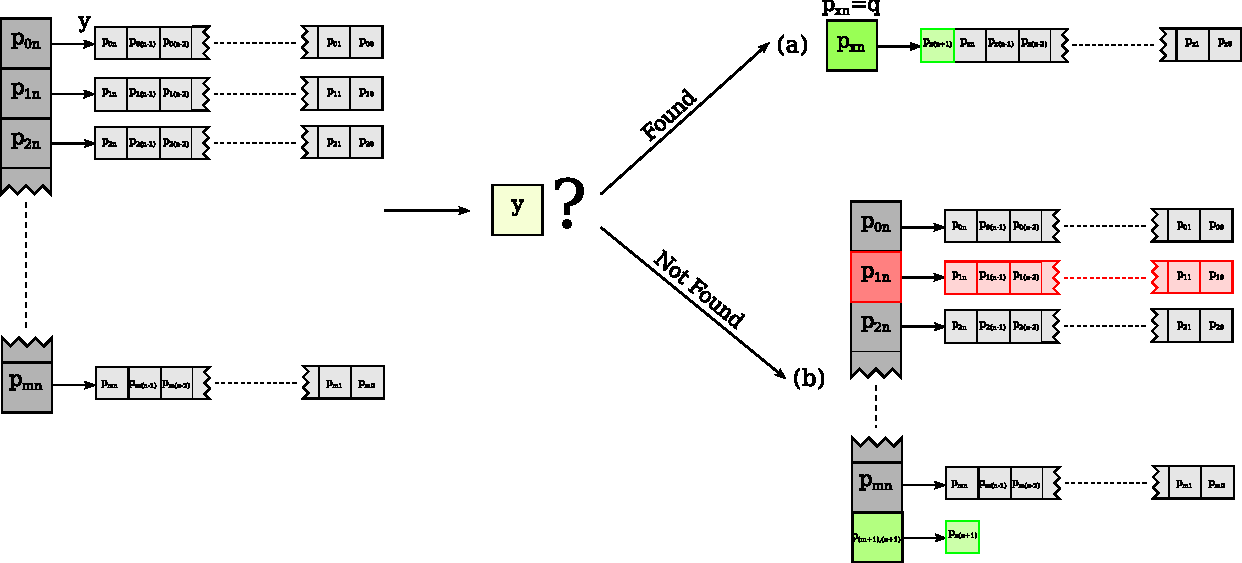
\includegraphics[width=\textwidth]{fig4.pdf}
%   \end{center}
% \end{frame}
% 
% \begin{frame}{Localization}
%   \begin{center}
%     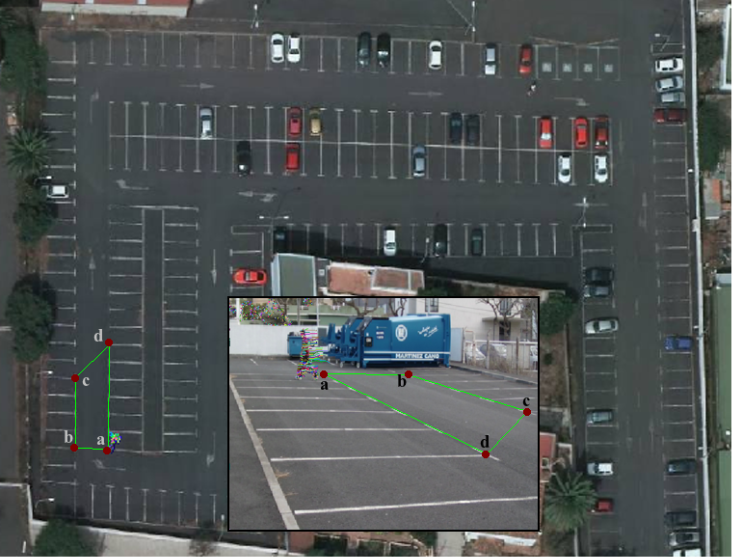
\includegraphics[height=0.7\textheight]{localization}
%   \end{center}
% \end{frame}

% \begin{frame}{Non-Rigid Contour Tracking}
%   \framesubtitle{Non-Rigid Contour Tracking}
%   \begin{center}
%     \includemovie[autoplay, repeat, controls]{\linewidth}{0.7\textheight}{/home/nestor/Seafile/Videos/Tesis/cp02/pipeline.mp4}
%   \end{center}
% \end{frame}

\begin{frame}{Non-Rigid Contour Tracking}
  \framesubtitle{Non-Rigid Contour Tracking}
  \begin{center}
    \includemovie[autoplay, repeat, controls]{0.75\linewidth}{.75\textheight}{/home/nestor/Seafile/Videos/Tesis/cp02/fgMaskAllFourMethods.mp4}
  \end{center}
\end{frame}

\begin{frame}{Non-Rigid Contour Tracking}
  \begin{columns}[c] % the "c" option specifies center vertical alignment
  \column{.5\textwidth} % column designated by a command
  \includemovie[autoplay, repeat, controls]{\linewidth}{.75\linewidth}{/home/nestor/Seafile/Videos/Tesis/cp02/trackingParking.mp4}
  \column{.5\textwidth}
  \includemovie[autoplay, repeat, controls]{\linewidth}{.75\linewidth}{/home/nestor/Seafile/Videos/Tesis/cp02/EPFL.mp4}
  \end{columns}
\end{frame}

\begin{frame}{Obstacle detection and tracking}
  \begin{itemize}
  \item Goals:
    \begin{enumerate}
      \item Good obstacle detection rate. \only<2->{\textcolor{green}{\cmark}}
      \item Obstacle localization. \only<3->{\textcolor{green}{\cmark}}
      \item Real time. \only<7->{\textcolor{orange}{\textbf{?}}}
      \item Environment conditions independence. \only<4->{\textcolor{green}{\cmark}}
      \item Tracking capabilities. \only<5->{\textcolor{green}{\cmark}}
      \item Moving cameras. \only<6->{\textcolor{red}{\xmark}}
    \end{enumerate}
  \end{itemize}
\end{frame}